\chapter{Partial Seed Set}\label{chapter:3}
Having discussed the easy regime (when SNR $>1$), we now shift our focus to the hard regime (SNR $\leq1$), which is the primary focus of this project. We aim to achieve the reconstruction efficiently when SNR $\leq1$ for the case of $k=2$ and then possibly generalise it to $k\geq 5$. However, by theorem \ref{thm:1.1.2}, some extra assistance is some additional assistance is required.\\
As highlighted in the introductory chapter, one of the main applications of community detection is to recover social circles in a given social network. In many cases, we have certain prior knowledge about a small subset of group members. These could be political leaders and their core supporters in a network based on political ideologies, or influencers and their most engaged followers in a celebrity fandom network. Therefore, a realistic setting for the extra information is that we are given a subset of vertices, which we call the \textit{partial seed set}, and our goal is to recover the labels of the remaining vertices.

\section{Problem Definition}
\begin{definition}[Partial Seed Set] \label{def: partial seed set}
    Let $(G, \sigma)$ be drawn from $SBM(n, k, \mathcal{P}),$ the partial seed set $R$ is a subset of vertices such that $\sigma_v$ is known for $\forall~v\in R,$ and $|R| = \alpha|V|$ for some $0<\alpha<1.$
\end{definition}
As outlined in the objectives chapter, given $(G, \sigma)$ drawn from $SSBM(n, k, \mathcal{P})$ with SNR $\leq1$ and a partial seed set $R$ with $|R|=\alpha|V|$ for some $0<\alpha<1,$ we aim to compute an assignment $\sigma': [n]\rightarrow \Omega$ efficiently that satisfies $\mathbb{E}(A(\sigma, \sigma'))> \mathbb{E}(A(\sigma, \sigma_{random}))=\frac{1-\alpha}{k}+\alpha,$ where $\sigma_{random}$ is the random guess.

\section{Greedy Recovery Algorithm}\label{sec: greedy recovery}
Since each vertex is more likely to connect with a vertex that belongs to the same community, if we assign the community label based on the most common community amongst a vertex's neighbours, then we have the hope to beat the random guess. Specially, for each $v\in V\setminus R,$ we assign it the most common label observed among its neighbours whose community labels are already known. This approach allows us to incrementally expand the set $R$ in a greedy fashion, continuing until no further assignments can be made. If there are any remaining unlabelled vertices, we then assigned them to one of the communities randomly. The steps of this algorithm are summarised in Algorithm \ref{algo2}.\\
\begin{algorithm}[H]\label{algo2} 
\SetKwInput{KwInput}{Input}                % Set the Input
\SetKwInput{KwOutput}{Output}              % Set the Output

\KwInput{Graph $G=(V, E)$ drawn from $SSBM(n, k, \mathcal{P}),$ and partial seed set $R$, which is a dictionary where keys are vertices and values are their corresponding community labels}
\KwOutput{Computed communities assignment $\sigma'$}
\SetKwFunction{FMain}{Greedy\_Recovery}
\SetKwProg{Fn}{Function}{:}{}
\Fn{\FMain{$G, R$}}{
\SetAlgoLined 
\LinesNumbered
\If{$|R| = |V|$}{\Return $R$;}
\For{$v \in V \setminus R$}{
  \If{$N(v)\cap R \neq \emptyset$}{$R[v]\gets$ the majority assignment of $v$'s neighbors;}
}
\Repeat{no new assignment can be made}{
\FMain{$G, R$}\Comment{greedily expand $R$}
}
\If{$\exists~v\notin R$}{$R[v]\gets\sigma_{random}(v)$;}
$\sigma'(v)\gets R[v]$ for $\forall~v\in V$;\\
\Return{$\sigma'$;}
}
\BlankLine
\caption{Greedy Recovery Algorithm}
\end{algorithm}
Therefore, the computed assignment $\sigma'$ consists of two subroutines: one is the greedy procedure, which we denote as $\sigma_{greedy}$, and the other is the random guess $\sigma_{random}$. Symbolically, let $\Gamma$ denote the set of vertices handled by the greedy procedures, then \begin{equation}\label{equn:3.1}
    \sigma'(v)=\begin{cases}
    \sigma(v)~&~\text{if}~v\in R\\
    \sigma_{greedy}(v)~&~\text{if}~v\in \Gamma\\
    \sigma_{random}(v)~&~\text{if}~v\in V\setminus(\Gamma\cup R)
    \end{cases}
\end{equation}
Algorithm \ref{algo2} has a running time of $\mathcal{O}(|V|^2|E|).$ This is because each recursive call to Greedy Recovery $(G, R)$ costs $\mathcal{O}(|V||E|)$ and increase the size of $R$ by at least 1, so there are at most n recursive calls. Therefore, Algorithm \ref{algo2} is clearly a polynomial time algorithm. \\
For sparse graph, particularly when $|E|<<|V|$, we can improve the running time by only checking the neighbours of vertices in $R$ during each iteration, instead of the entire vertex set. This optimisation leads to Algorithm \ref{algo3}, which has a running time of $\mathcal{O}(|E|^2|V|).$\\
\begin{algorithm}[H]\label{algo3}
\caption{Faster Greedy Recovery Algorithm}
\DontPrintSemicolon % Remove semicolon at the end of each line
\KwIn{Graph $G = (V, E)$ and $R$}
\KwOut{$\sigma'$}
\SetKwFunction{FMain}{Faster\_Greedy\_Recovery}
\SetKwProg{Fn}{Function}{:}{\KwRet}
\Fn{\FMain{$G, R$}}{
\LinesNumbered
\SetAlgoLined 
  \If{$|R| = |V|$}{
    \KwRet $R$\;
  }
  $Q \gets$ empty queue\;
  \For{$v \in R$}{
    Enqueue $v$ into $Q$\;
  }
  \While{$Q$ is not empty}{
    $v \gets Q$.dequeue()\;
    \For{$u \in N(v) \setminus R$}{
      $R[u] \gets \text{the majority assignment of } u\text{'s neighbors}$\;
      Enqueue $u$ into $Q$\;
    }
  }
  \If{$\exists~v\notin R$}{$R[v]\gets\sigma_{random}(v)$}
  $\sigma'(v)\gets R[v]$ for $\forall~v\in V$\\
  \KwRet $\sigma'$\;
}
\BlankLine
\end{algorithm}

\section{Analysis}
We adopt the same notations as those introduced in Equation \ref{equn:3.1}.
\begin{lemma}\label{lemma1}
    Let $(G, \sigma)$ be drawn from $SSBM(n, k, p_{in}, p_{out}),$ with a partial seed set $R$ such that $|R|=\alpha\cdot n$ for some $\alpha\in(0,1).$ Let $\sigma'$ be the assignment computed by our greedy recovery algorithm. If for each vertex $v\in\Gamma,$ $\mathbb{P}(\sigma(v)=\sigma_{greedy}(v))>\frac{1}{k},$ then $\mathbb{E}({A(\sigma, \sigma'}))>\frac{1-\alpha}{k}+\alpha.$
\end{lemma}
\begin{proof}
 We know for vertex $v\in V\setminus(\Gamma\cup R),$ $\mathbb{P}(\sigma_v=\sigma_v')=\mathbb{P}(\sigma(v)=\sigma_{random}(v))=1/k,$ and for each $v\in R,$ $\mathbb{P}(\sigma_v=\sigma_v')=\mathbb{P}(\sigma(v)=\sigma(v))=1.$ If $\mathbb{P}(\sigma_v=\sigma_v')>1/k$ for $v\in\Gamma,$ then $\mathbb{E}(\sum_V\mathbb{1}(\sigma_v=\sigma_v'))=\sum_V\mathbb{E}(\mathbb{1}(\sigma_v=\sigma_v'))=\sum_V\mathbb{P}(\sigma_v=\sigma_v')=\sum_\Gamma\mathbb{P}(\sigma(v)=\sigma_{greedy}(v))+\sum_{V\setminus(\Gamma\cup R)}\mathbb{P}(\sigma(v)=\sigma_{random}(v))+\sum_{R}\mathbb{P}(\sigma_v=\sigma_v)\\>|\Gamma|\frac{1}{k}+|V\setminus(\Gamma\cup R)|\frac{1}{k}+|R|=\frac{1}{k}(n-\alpha n)+\alpha n,$ so $\mathbb{E}({A(\sigma, \sigma'}))>\frac{1-\alpha}{k}+\alpha.$
\end{proof}
For $v\in\Gamma,$ let $R_v$ denote the set of neighbours of v whose assignments have already been determined at the time our greedy algorithm evaluates vertex $v.$ Let $\Re_v$ denote the set of vertices in $R_v$ that belong to the most common community among $v$'s neighbours when greedy algorithm examines v. So, $\Re_v\subseteq N(v)\cap R_v$ and $\sigma_v'=\sigma_u'$ for any $u\in\Re_v$
\begin{claim}\label{claim2}
     Let $(G, \sigma)$ be drawn from $SSBM(n, k, p_{in}, p_{out})$, and $\sigma'$ be the assignment computed by our greedy recovery algorithm. If $SNR>0$ (i.e., $p_{in}>p_{out}$)\footnote{As we only care about the associativity case.} and $|\Re_v|>max(0,~1-\frac{log(|\Re_v|)}{log(1-1/k)}),$ then $\mathbb{P}(\sigma_v=\sigma_v')>\frac{1}{k}$~~for all $v\in\Gamma.$
\end{claim}
\begin{proof}
    Suppose $(v_1, v_2, \ldots, v_{|\Gamma|})$ is the sequence of vertices examined by $\sigma_{greedy}$. we induct on the index of the vertices in this sequence. Let $e_{out}$ denote the edge with endpoints in different communities.\\
    For $v_1,$ \begin{align*}
    \mathbb{P}(\sigma_{v_1}\neq\sigma_{v_1}')&=\mathbb{P}(\sigma_{v_1}\neq\sigma_{v_1}'|\sigma_u=\sigma_u'~\text{for any u in}~\Re_{v_1})\\
    &\leq\mathbb{P}(\{v_1, u\}~\text{is}~e_{out}~\text{for any}~u\in\Re_{v_1}~|~\{v_1, u\}\in E~\text{for any}~u\in\Re_{v_1})\\
    &=(\frac{p_{out}}{p_{in}+p_{out}})^{|\Re_{v_1}|}\\
    &<(1-\frac{1}{k})^{|\Re_{v_1}|} ~~~~~~~\text{as}~(\frac{p_{out}}{p_{in}+p_{out}})<\frac{1}{2}\leq(1-\frac{1}{k})\\
    &<(1-\frac{1}{k})
    \end{align*}
    Now, consider some $v_{i>1}$ in this sequence of vertices. Let $A:=$ the event that $\sigma_{v_i}\neq\sigma_{v_i}'$, $B_j:=$ the even that $j$ vertices in $\Re_{v_i}$ are labelled incorrectly. \begin{align*}
    \mathbb{P}(\sigma_{v_i}\neq\sigma_{v_i}')&=\sum_{j=0}^{|\Re_{v_i}|}\mathbb{P}(\sigma_{v_i}\neq\sigma_{v_i}'\cap j~\text{vertices in}~\Re_{v_i}~\text{labelled incorrectly})\\
    &=\sum_{j=0}^{|\Re_{v_i}|}\mathbb{P}(A|B_j)\mathbb{P}(B_j)
    \end{align*}
Now, \begin{align*}
    \mathbb{P}(A|B_j)&\leq\mathbb{P}((|\Re_{v_i}|-j)~\text{edges are }~e_{out}~\text{among all edges between }~v_i~\text{and}~\Re_{v_i})\\
    &=(\frac{p_{out}}{p_{in}+p_{out}})^{|\Re_{v_i}|-j}\\
    &<(1-\frac{1}{k})^{|\Re_{v_i}|-j}
\end{align*} 
Also by inductive hypothesis, $\mathbb{P}(B_j)<(1-\frac{1}{k})^j,$ and since $|\Re_v|>1-\frac{log(|\Re_v|)}{log(1-1/k)},$ we have $|\Re_v|(1-\frac{1}{k})^{|\Re_v|}<1-\frac{1}{k}$.\\Hence,
\begin{align*}
    ~~~~~~~~\mathbb{P}(\sigma_{v_1}\neq\sigma_{v_1}')&=\sum_{j=0}^{|\Re_{v_i}|}\mathbb{P}(A|B_j)\mathbb{P}(B_j)\\
    &<\sum_{j=0}^{|\Re_{v_i}|}(1-\frac{1}{k})^j\cdot(1-\frac{1}{k})^{|\Re_{v_i}|-j}\\
    &=|\Re_{v_i}|(1-\frac{1}{k})^{|\Re_{v_i}|}\\
    &<1-\frac{1}{k}
\end{align*}
Therefore, we have shown that $\mathbb{P}(\sigma_{v}\neq\sigma_{v}')<1-1/k$~for~$v\in\Gamma \Rightarrow\mathbb{P}(\sigma_{v}=\sigma_{v}')>1/k$~for~$v\in\Gamma.$
\end{proof}
\begin{corollary}
     Let $(G, \sigma)$ be drawn from $SSBM(n, k, p_{in}, p_{out}),$ $|R|=\alpha\cdot n$ for some $\alpha\in(0,1),$ and $\sigma'$ be the assignment computed by our greedy recovery algorithm. If $SNR>0$ and$|\Re_v|>max(0,~1-\frac{log(|\Re_v|)}{log(1-1/k)}),$ then $\mathbb{E}({A(\sigma, \sigma'}))>\frac{1-\alpha}{k}+\alpha,$~i.e., our greedy recovery algorithm is strictly better than random guess in expectation.
\end{corollary}
\begin{proof}
    By Lemma \ref{lemma1} and Claim \ref{claim2}.
\end{proof}
\begin{remark}
    for $k=2$, $|\Re_v|>2$ would be sufficient.
\end{remark}
\section{Experimental Results for k=2 in Hard Regime}
In this section, we delve into the empirical results of the greedy recovery algorithm for the case of 2 communities.
\subsection{Spare Graph}
\begin{figure}[H]
    \centering
    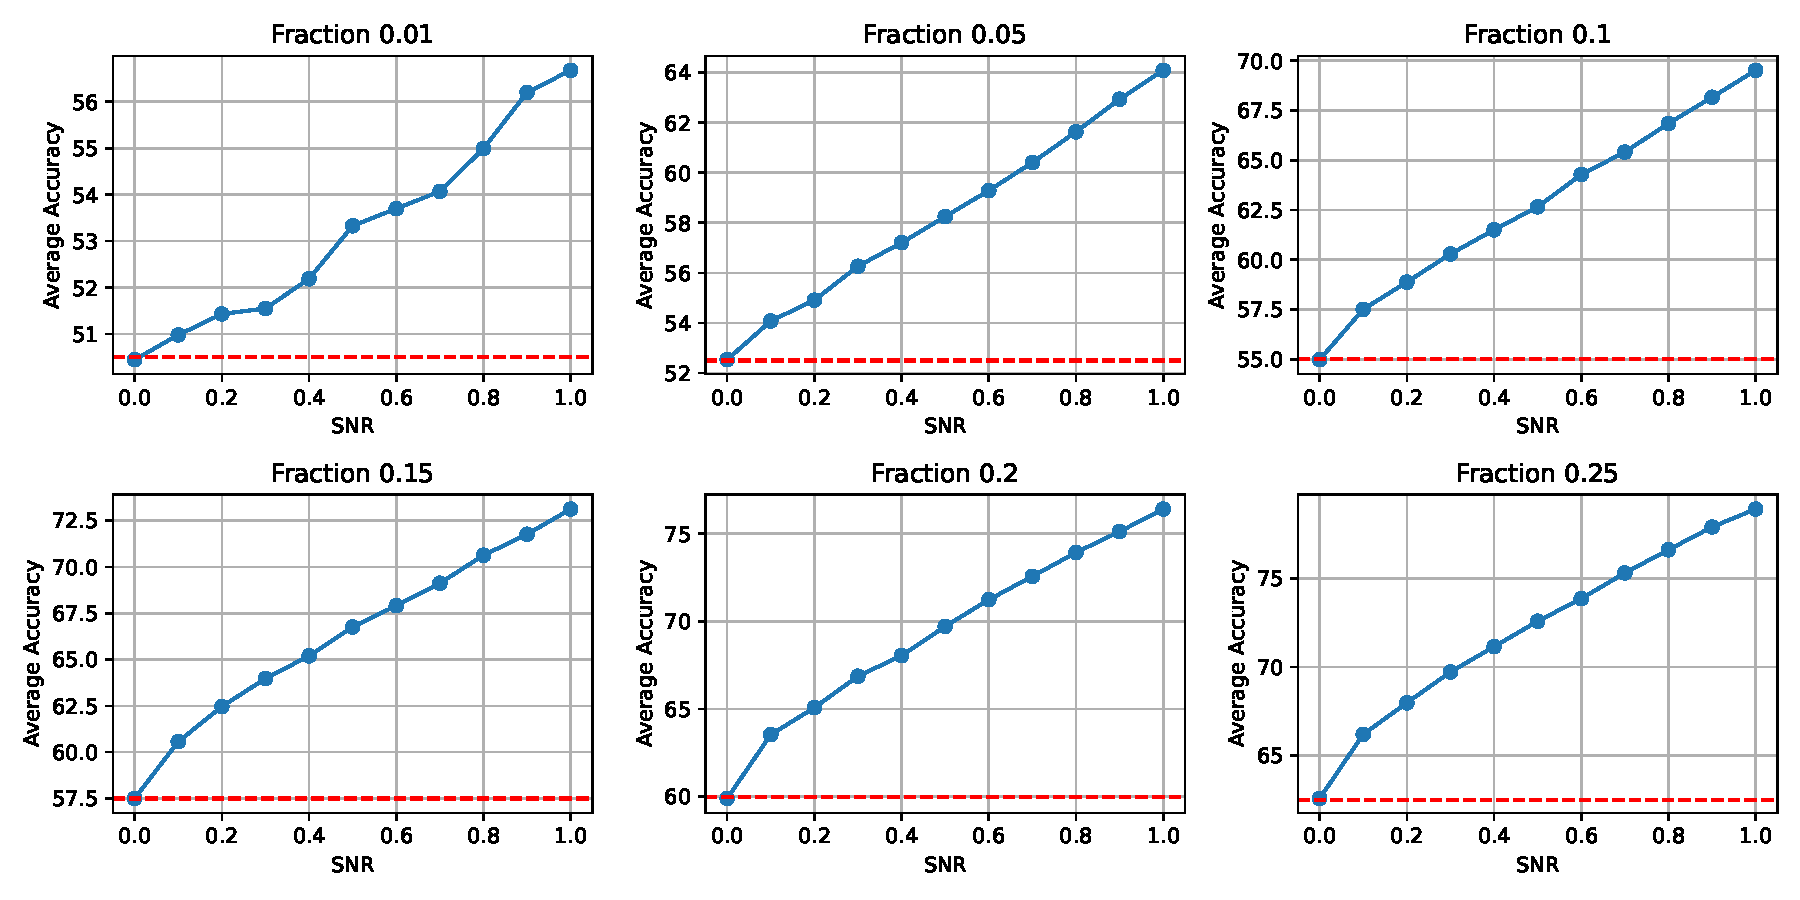
\includegraphics[width=1\linewidth]{Figures/Greedy_Recovery_Sparse_50000_1.pdf}
    \caption[Accuracy of Greedy Recovery Algorithm in Sparse Graph with $k=2$]{The blue line represents the accuracy of greedy recovery algorithm across different fraction values $\alpha$ (recall $\alpha$ in definition \ref{def: partial seed set}) for SNR ranging from 0 to 1. The red dashed line represents the accuracy of random guess($=\frac{1-\alpha}{2}+\alpha$) for a given fraction value $\alpha$. For instance, the first plot is the accuracy of our algorithm and the random guess when $|R|=0.01\cdot|V|.$ The experiment results\protect\footnotemark are averaged over 10 instances with $n=10^5$ and $c=3.$}
    \label{fig:greedy_sparse}
\end{figure}
\footnotetext{The parameters chosen for the sparse graph are in alignment with those used in \cite{the_non-backtracking}.}
From figure \ref{fig:greedy_sparse}, we observe that when SNR $>0$, our greedy recovery algorithm perform noticeably better than the random guess  for all the tested fraction values $\alpha.$\\
\begin{figure}[ht]
    \centering
    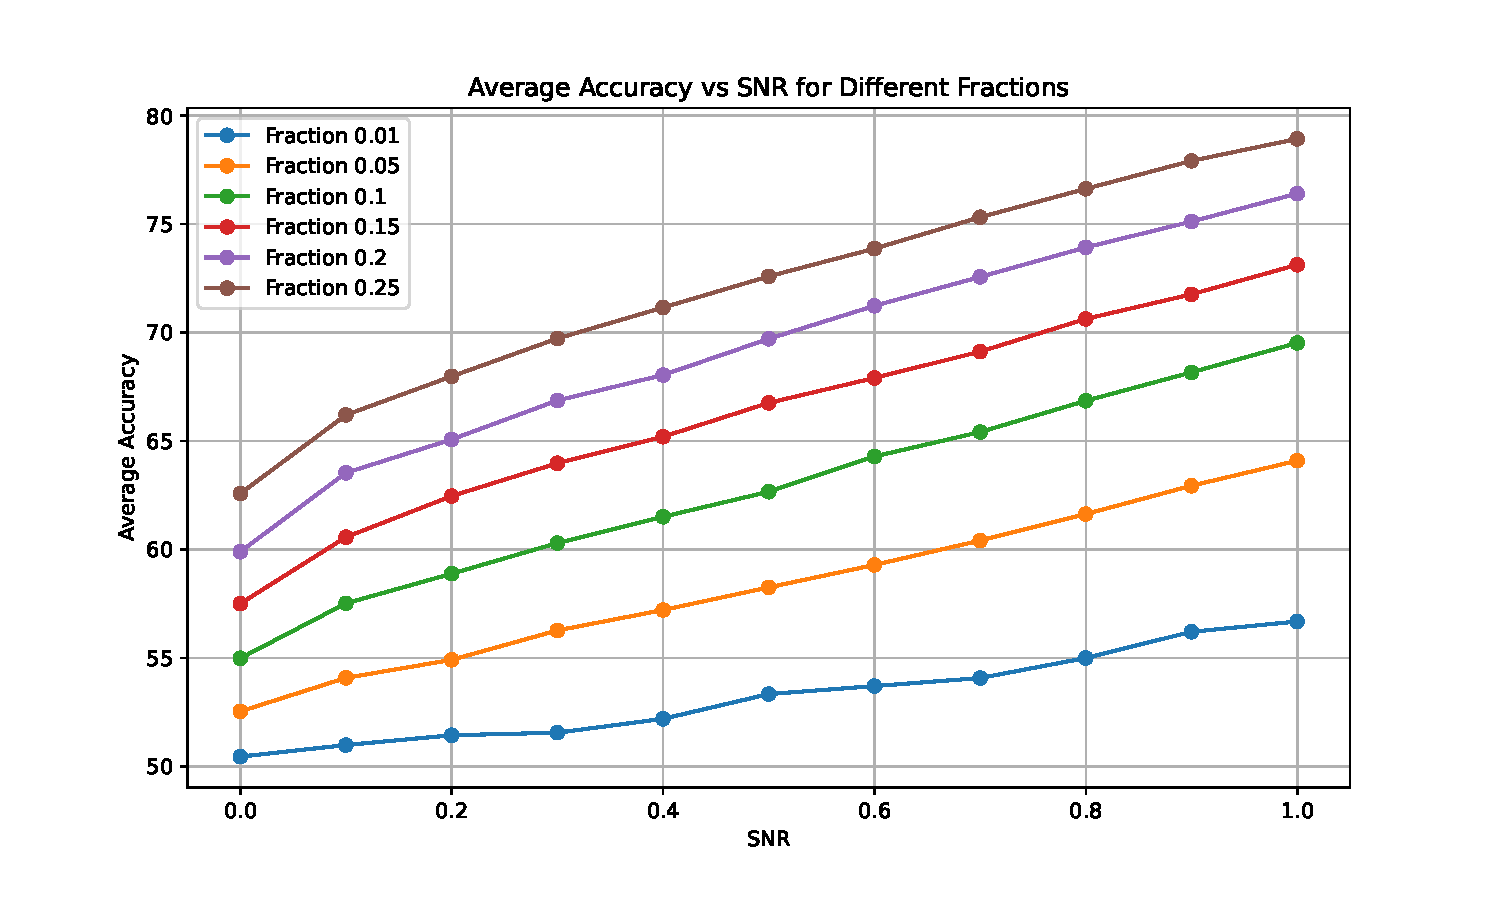
\includegraphics[width=1\linewidth]{Figures/Greedy_Recovery_Sparse_50000_2.pdf}
    \caption[A Compact Version of Accuracy Plot]{This plot combines the results from Figure \ref{fig:greedy_sparse} into a single compact visualisation.}.
    \label{fig: compact_sparse}
\end{figure}
From figure \ref{fig: compact_sparse}, we observe that the accuracy of the greedy recovery algorithm improves as the SNR increases, indicating that our algorithm performs better when the community structure becomes more apparent, which aligns with our expectations,
\subsection{Dense Graph}
\begin{figure}[H]
    \centering
    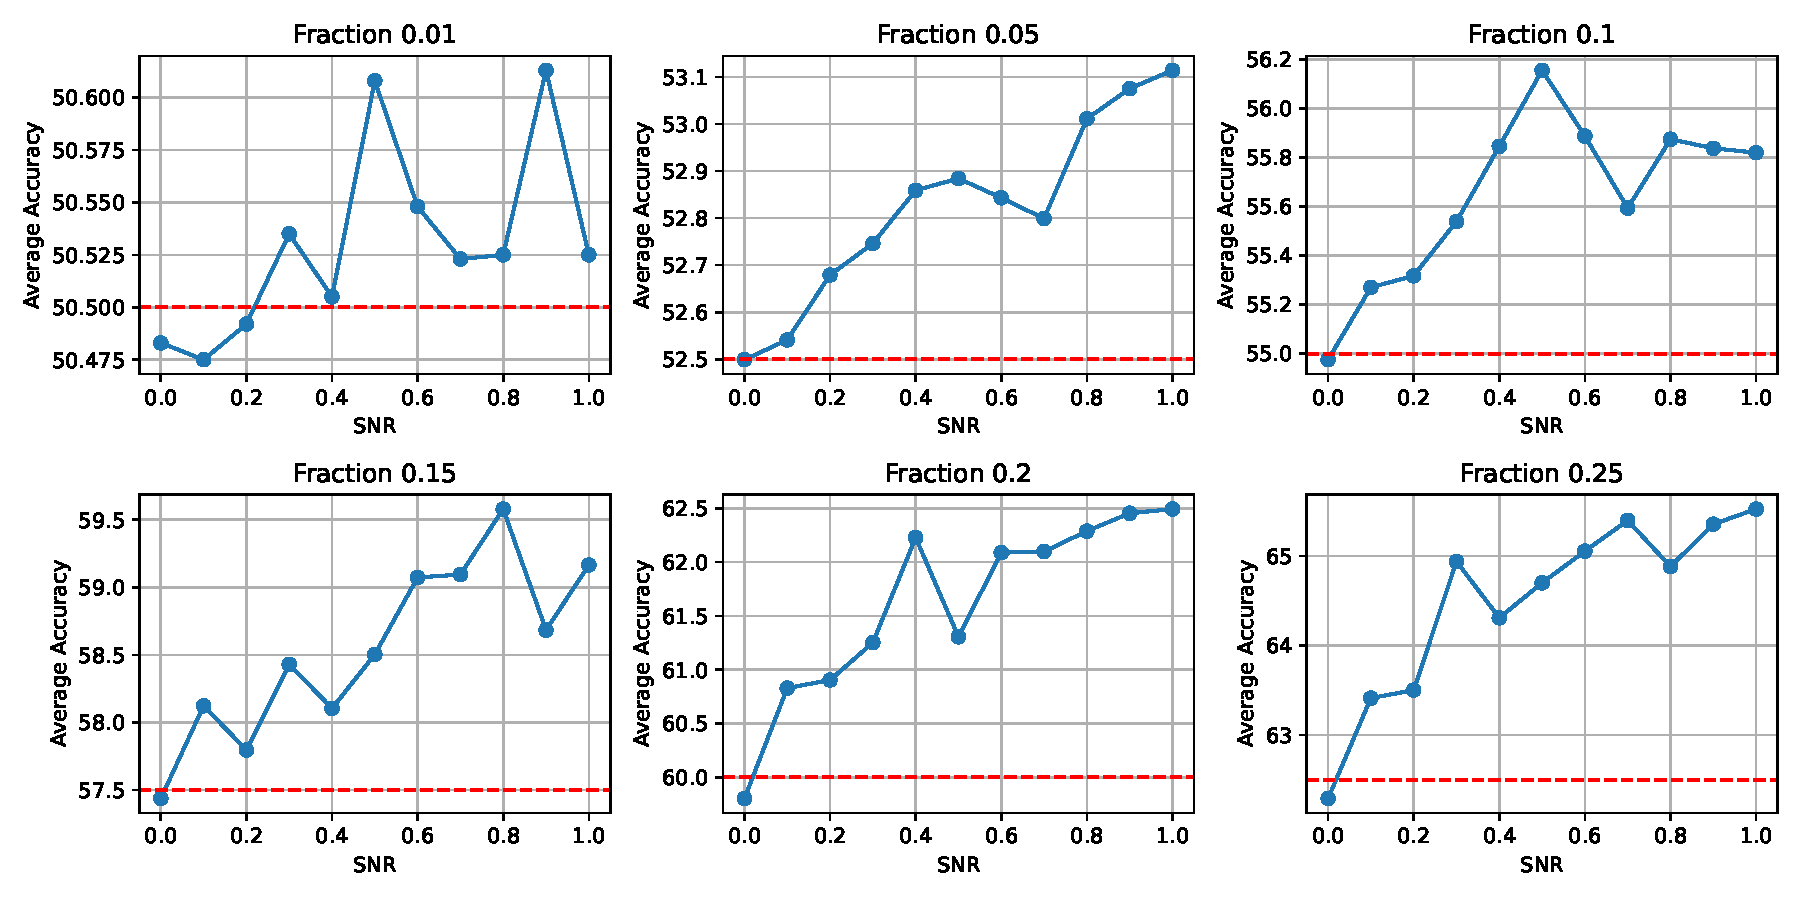
\includegraphics[width=1\linewidth]{Figures/Greedy_Recovery_super_dense_3.pdf}
    \caption[Accuracy of Greedy Recovery Algorithm in Dense Graph with $k=2$]{The blue line represents the accuracy of greedy recovery algorithm across different values of $\alpha$(=fraction) for SNR ranging from 0 to 1. The red dashed line represents the accuracy of random guess($=\frac{1-\alpha}{2}+\alpha$) for a given fraction value $\alpha$. The experiment results\protect\footnotemark are averaged over 10 instances with $n=10^4$ and $c=200.$}
    \label{fig:greedy_dense}
\end{figure}
\footnotetext{The parameters chosen for the dense graph are in alignment with those used in \cite{dallamico:tel-03454227}.}
This time, the pattern observed in figure \ref{fig:greedy_dense} is more fluctuating, and the situation is more subtle. Our greedy recovery algorithm generally suppress the random guess, but its superiority is not consistent, particularly when fraction value and SNR are small.\\
This is possibly due to the fact that the set $R$ is small in the early stage, so the greedy algorithm is assigning labels based on only a small fraction of each vertex's neighbours, which may cause our greedy algorithm to underperform compared to random guessing. Moreover, the detrimental effects of these incorrect assignments could be magnified in later stages, leading to fluctuations in the accuracy of our greedy algorithm.
\clearpage
\subsection{Heuristic Improvement}
One potential remedy to the issue encountered in the dense graph is to delay the assignment of a vertex until we have sufficient information about it. Specially, for each vertex,  we determine its label only when a certain fraction, say $h,$  of its neighbours is known to us, i.e., $|R\cap N(v)|>h.$ This criterion ensures that our greedy recovery algorithm expands the set $R$ by prioritising vertices for which we have a higher confidence in their labelling. As $R$ grows, we expect the algorithm to accumulate more information about the vertices that were skipped in earlier stages. Consequently, this algorithm should have a higher chance of computing a correct assignment when revisiting these vertices compared to the original approach. Therefore, it is reasonable to expect the modified algorithm to outperform the original greedy recovery algorithm. The steps for this heuristic greedy recovery algorithm are outlined in Algorithm \ref{algo4}.
\clearpage
\begin{algorithm}[H]\label{algo4}
\SetKwInput{KwInput}{Input}                % Set the Input
\SetKwInput{KwOutput}{Output}              % Set the Output
\KwInput{$G, R$ and the heuristic factor $h$}
\KwOutput{Computed communities assignment $\sigma'$}
\SetKwFunction{FMain}{Heuristic\_Greedy\_Recovery}
\SetKwProg{Fn}{Function}{:}{}
\Fn{\FMain{$G, R, h$}}{
\SetAlgoLined 
\LinesNumbered
\If{$|R| = |V|$}{\Return $R$;}
\For{$v \in V \setminus R$}{
  \If{$N(v)\cap R > h$}{$R[v]\gets$ the majority assignment of $v$'s neighbors;}
}
\Repeat{no new assignment can be made in this heuristic way}{
\FMain{$G, R, h$}\Comment{greedily grow $R$}
}
$\sigma'\gets$ Greedy\_Recovery(G, R)\\
\Return{$\sigma'$;}
}
\BlankLine
\caption{Heuristic Greedy Recovery Algorithm}
\end{algorithm}
\clearpage
The following figures present experimental results demonstrating the performance of the heuristic improvement for dense graphs. 
\begin{figure}[H]
    \centering
    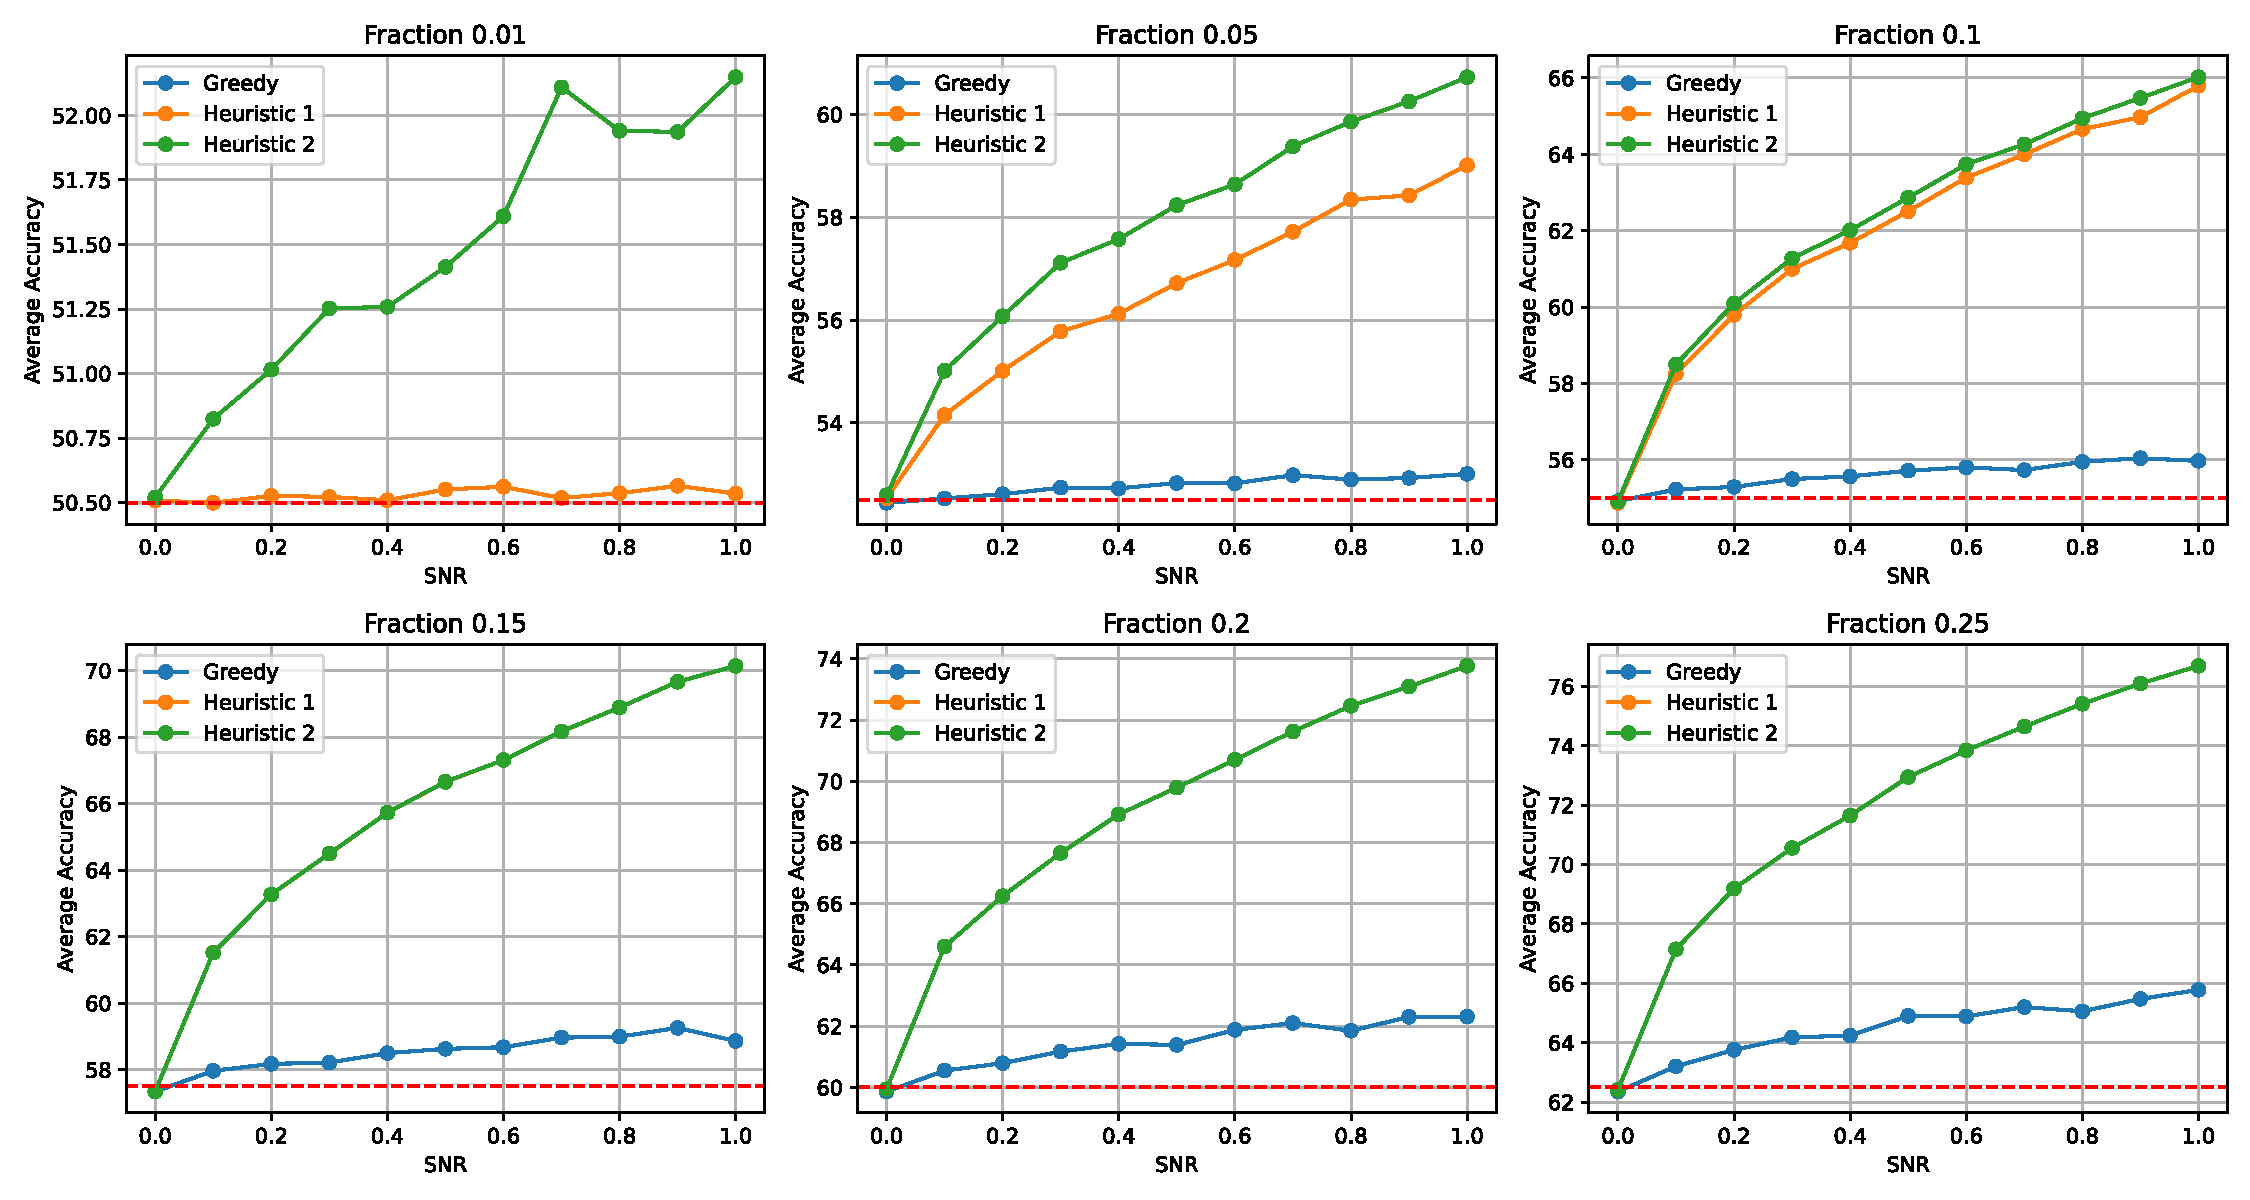
\includegraphics[width=1\linewidth]{Figures/heu_super_dense.pdf}
    \caption[Accuracy of Greedy Recovery Algorithm versus Heuristic Strategy with 2 Different Factors for $k=2$.]{As usual, the red dashed line represents the accuracy of random guess, while blue line represents the accuracy of greedy recovery algorithm. The orange and green lines represent the accuracy of the greedy recovery algorithm with heuristic factors $h=\sqrt{c}$ and $h=\log{c}$, respectively. The experiment results are averaged over 10 instances with $n=10^4$ and $c=200.$}
    \label{fig: heuristic greedy}
\end{figure}
It is noteworthy that in Figure \ref{fig: heuristic greedy}, when the fraction value is 0.01, the accuracy of Heuristic 1 is identical to the accuracy of the greedy recovery algorithm, causing the blue line to be covered by the orange line in plot 1. As the fraction value increases, the accuracy of Heuristic 1 converges to the accuracy of Heuristic 2.  Therefore, in the plots for fraction value $=0.15,$ $0.2$ and $0.25,$ the orange line is covered by the green line.\\
Moreover, we can observe that the greedy recovery algorithm with heuristic factor $h=\log{c}$ improves the accuracy of the original greedy algorithm by up to 12\% at SNR $=1$ in the plot of fraction value $=0.2.$ Furthermore, this enhanced algorithm consistently outperforms the random guess across all the selected fraction values when SNR $>0$.


